\chapter{Chapter Three}

\section{Event Comparisons}
Now, we consider each of the selected events individually, demonstrating that the events were
classified correctly, and breaking down the results from each case. Although it is nearly impossible to
extricate lake influence from synoptically classified events, synoptic-scale ascent is considered the
characterizing factor. Descriptions of the synoptic pattern during each event are given without
reference; For reference, see Appendix A for the 500mb Geopotential Heights, Skew-T charts, and
Sounding Climatology utilized. These descriptions are ancillary to the study and are provided to
demonstrate a variety of patterns are represented.

\begin{figure}[p]
\includegraphics[width=\textwidth]{grid/ref/20140118}
\caption{Gridded $Z_{eH}$ comparison for 18 January 2014. Time-average of all admitted scans.} 
\label{fig:grid_ref_20140118}
\end{figure}

\begin{figure}[p]
\includegraphics[width=\textwidth]{grid/zdr/20140118}
\caption{Gridded $Z_{DR}$ comparison for 18 January 2014. Time-average of all admitted scans.} 
\label{fig:grid_zdr_20140118}
\end{figure}


\subsection{18 January 2014 - Synoptic}
In this event, a weak shortwave is approaching Southern Ontario as it rounds the base of a longwave
trough centered over the Eastern US. With the study area in the attendant
region of upper-level divergence, and a moist column present through 500mb, 
scattered snow showers form ahead of the shortwave. Figure \ref{fig:grid_ref_20140118} depicts
similiar cellular patterns between radars in the time-averaged $Z_{eH}$ field. In contrast, the $Z_{DR}$
comparison in Figure \ref{fig:grid_zdr_20140118}
shows that although the fields are similiar in their anisotropy, the spatial matching between the two is
tenuous everywhere but in the heaviest showers. To
investigate further, we examine a scatter-plot directly comparing matched values between radars.
Artifacts are present in both moments in Figure
\ref{fig:scatter_20140118}, indicated by evenly spaced vertical lines; these indicate an anomaly
originating from the axis of which they are normal to. For
$Z_{eH}$, Figure \ref{fig:scatter_ref_20140118} shows that artifacts are no longer present for values
greater than 15 dBZ, which indicates that a
stronger weather signal leads to better matching. On the contrary, Figure \ref{fig:scatter_zdr_20140118}
shows that for $Z_{DR}$, artifacts are present throughout. 

\begin{figure}[H]
\centering
   \begin{subfigure}{0.49\linewidth} \centering
     \includegraphics[scale=0.38]{scatter/ref/20140118}
     \caption{$Z_{eH}$ (dBZ)}\label{fig:scatter_ref_20140118}
   \end{subfigure}
   \begin{subfigure}{0.49\linewidth} \centering
     \includegraphics[scale=0.38]{scatter/zdr/20140118}
     \caption{$Z_{DR}$ (dB)}\label{fig:scatter_zdr_20140118}
   \end{subfigure}
\caption{Direct comparisons for 18 January 2014. Dataset includes all admitted grid cells.} \label{fig:scatter_20140118}
\end{figure}

\begin{figure}[H]
\includegraphics[width=0.75\textwidth]{hist/20140118}\centering
\caption{Histograms of $Z_{DR}$ (left), $Z_{DR}$ bias at CWKR, determined by subtracting the gridded, bias adjusted $Z_{DR}$ at KBUF from the $Z_{DR}$ at
CWKR. Both datasets exclude matched points with KDE $< 2$. } 
\label{fig:hist_20140118}
\end{figure}

It is still possible to extract a signal from the noise though, by excluding data points with a
normalized kernel density less than two. These points are used to resolve the bias present in
$Z_{DR}$, as suggested by the comparisons. Figure \ref{fig:hist_20140118} gives an estimate of the
bias at CWKR by using this method and the known bias at KBUF as provided by the NEXRAD
External Target Bias Estimation technique. This method yields a value of -0.095 dB, which when
considered with the error threshold of $\pm$0.1 dB, indicates no discernible bias at CWKR.




\begin{figure}[p]
\includegraphics[width=\textwidth]{grid/ref/20140123}
\caption{Gridded $Z_{eH}$ comparison for 23 January 2014. Time-average of all admitted scans.} 
\label{fig:grid_ref_20140123}
\end{figure}

\begin{figure}[p]
\includegraphics[width=\textwidth]{grid/zdr/20140123}
\caption{Gridded $Z_{DR}$ comparison for 23 January 2014. Time-average of all admitted scans.} 
\label{fig:grid_zdr_20140123}
\end{figure}

\subsection{23 January 2014 - Lake-Effect}
A positively tilted longwave trough dominates the eastern third of Canada during this event, with NW
winds at 850mb and SW winds at the surface. This light yet convergent flow yields the single, heavy
band depicted in Figure \ref{fig:grid_ref_20140123}, colloquially referred to as ``tea-kettle'' lake-effect
snow. There is also a background stream of very light lake-effect snow impinging from Lake Erie.
Spatial banding patterns of the lake-effect snow in the time-averaged $Z_{eH}$ fields as compared 
between the radars are remarkably similar. The difference between the grid mean values are within only
0.13 dBZ. In contrast, the $Z_{DR}$ comparison indicates that
although the fields are similiar in their anisotropy, the spatial matching between the two is tenuous
everywhere but in the heaviest showers.  An anistropic pattern is also imparted on the $Z_{DR}$ fields
by the light snow from Lake Erie, evident in Figure \ref{fig:grid_zdr_20140123}. 
The scatter-plot in Figure \ref{fig:scatter_ref_20140123} shows an analysis free of artifacts, and good
agreement on average between radars. Although the agreement in $Z_{eH}$ between radars as
indicated by the orthonormal regression is acceptable, the chi-square
statistic indicates a high error variance.  Both analysis methods have indicated bias in $Z_{DR}$, so the
kernel density method for estimating bias is used. Figure \ref{fig:hist_20140123} shows an estimate of
the bias at CWKR, with a value of -0.055 dB. Once again, no discernible bias exists outside of the error
threshold of $\pm$0.1 dB for this event.

\begin{figure}[H]
\centering
   \begin{subfigure}{0.49\linewidth} \centering
     \includegraphics[scale=0.38]{scatter/ref/20140123}
     \caption{$Z_{eH}$ (dBZ)}\label{fig:scatter_ref_20140123}
   \end{subfigure}
   \begin{subfigure}{0.49\linewidth} \centering
     \includegraphics[scale=0.38]{scatter/zdr/20140123}
     \caption{$Z_{DR}$ (dB)}\label{fig:scatter_zdr_20140123}
   \end{subfigure}
\caption{Direct comparisons for 23 January 2014. Dataset includes all admitted grid cells.}
\label{fig:scatter_20140123}
\end{figure}

\begin{figure}[H]
\includegraphics[width=0.75\textwidth]{hist/20140123}\centering
\caption{Histograms of $Z_{DR}$ (left), $Z_{DR}$ bias at CWKR, determined by subtracting the
gridded, bias adjusted $Z_{DR}$ at KBUF from the $Z_{DR}$ at CWKR. Both datasets exclude
matched points with KDE $< 2$. } 
\label{fig:hist_20140123}
\end{figure}

\subsection{1 February 2014 - Synoptic}
This event is characterized by strong SW flow aloft, with above average moisture content. This leads to
widespread stratiform snow, with an eventual transition to rain outside of the time interval selected.

\begin{figure}[H]
\includegraphics[width=\textwidth]{grid/ref/20140201}
\caption{Gridded $Z_{eH}$ comparison for 1 February 2014. Time-average of all admitted scans.} 
\label{fig:grid_ref_20140201}
\end{figure}

\begin{figure}[H]
\includegraphics[width=\textwidth]{grid/zdr/20140201}
\caption{Gridded $Z_{DR}$ comparison for 1 February 2014. Time-average of all admitted scans.} 
\label{fig:grid_zdr_20140201}
\end{figure}
 A large swath of steady snow is depicted by the time-averaged $Z_{eH}$ in Figure
 \ref{fig:grid_ref_20140201}. Furthermore, Figure \ref{fig:grid_zdr_20140201} shows smoother $Z_{DR$
 fields as compared with other events, which confirms the stratiform nature of the precipitation. Next, Figure \ref{fig:scatter_20140201} indicates good agreement with low error variance. 
 
 \begin{figure}[H]
\centering
   \begin{subfigure}{0.49\linewidth} \centering
     \includegraphics[scale=0.38]{scatter/ref/20140201}
     \caption{$Z_{eH}$ (dBZ)}\label{fig:scatter_ref_20140201}
   \end{subfigure}
   \begin{subfigure}{0.49\linewidth} \centering
     \includegraphics[scale=0.38]{scatter/zdr/20140201}
     \caption{$Z_{DR}$ (dB)}\label{fig:scatter_zdr_20140201}
   \end{subfigure}
\caption{Direct comparisons for 1 February 2014. Dataset includes all admitted grid cells.} \label{fig:scatter_20140201}
\end{figure}
